\setchapterpreamble[u]{\margintoc}
\chapter{Models}
\labch{models}
After the previous two chapters focused on basic ideas and mathematics behind neural networks, this chapter will introduce basic model architectures and building blocks of many neural networks.
Not every new publication reinvents the wheel and often the repeated use of merited building blocks can be observed.

It is particularly interesting that most networks make a single choice for a basic building block throughout the network.
The choice affects the properties of convolution, normalization and activation layers as a sequence of these makes up such a block.
Mainly, parameters like kernel size, normalization function and activation function are picked beforehand and remain the same for the entire network.
Arguably, one could say, that it shows some similarities to the way network motifs make up networks~\cite{uri_alon}.

However, the focus of this chapter is the introduction of advanced model architectures like adversarial models or autoencoder.
To aid this cause, this chapter starts with simpler architectures.

\section{Discriminators \& Classifiers}
Discriminators and Classifiers are prime examples in many books which deal with neural networks.
Both architectures are designed to take high-dimensional inputs and produce low-dimensional outputs from these.
These outputs then represent a class prediction. \\
For discriminators these class predictions only include two classes (often 'real' or 'fake').
Thus, both often display the same architecture.

Probably the most common architecture is the VGG-architecture.
This architecture was developed for the ImageNet classification challenge~\cite{imagenet}.
\marginnote{ImageNet consists of 15 million high-resolution images in 22,000 categories.
A subset of 1.2 million $256 \times 256 $ pixel images in 1,000 categories is used for the ILSVR challenge.
VGG16 was runner-up in ILSVRC-2014.}
The VGG network exists in different variants, which feature differing numbers of layers.
VGG16, for instance, features 16 layers with weights.\\
VGG16 is exemplary for many classifier structures, as the spatial resolution is slowly reduced while the number of channels increases at the same time.
This does not happen continuously but in a step-wise manner.
After every two or three blocks (convolutional layer + activation layer) there is a pooling layer which reduces the resolution by $\frac{1}{2}$ along each axis~\cite{VGG}.
Every time the resolution is reduced by $\frac{1}{4}$ the number of kernels for the following convolutions is doubled.
In the end there are a couple fully connected layers which interpret the final features and generate a prediction.
\reffig{VGG} shows the networks architecture.
\todo{reinsert this figure}
%\begin{figure}
%    \begin{tikzpicture}
\tikzstyle{connection}=[ultra thick,every node/.style={sloped,allow upside down},draw=\edgecolor,opacity=0.7]
%%%%%%%%%%%%%%%%%%%%%%%%%%%%%%%%%%%%%%%%%%%%%%%%%%%%%%%%%%%%%%%%%%%%%%%%%%%%%%%%%%%%%%%%
%% Draw Layer Blocks
%%%%%%%%%%%%%%%%%%%%%%%%%%%%%%%%%%%%%%%%%%%%%%%%%%%%%%%%%%%%%%%%%%%%%%%%%%%%%%%%%%%%%%%%
% conv1_1,conv1_2
\pic[shift={(0,0,0)}] at (0,0,0) {RightBandedBox={name=cr1,caption=conv1,%
        xlabel={{"64","64"}},ylabel=224,zlabel=224,fill=\ConvColor,bandfill=\ConvReluColor,%
        height=40,width={2,2},depth=40}};
%pool1
\pic[shift={(0,0,0)}] at (cr1-east) {Box={name=p1,%
        fill=\PoolColor,opacity=0.5,height=35,width=1,depth=35}};
%%%%%%%%%%
% conv2_1,conv2_2
\pic[shift={(2,0,0)}] at (p1-east) {RightBandedBox={name=cr2,caption=conv2,%
        xlabel={{"128","128"}},zlabel=112,fill=\ConvColor,bandfill=\ConvReluColor,%
        height=35,width={3,3},depth=35}};
%pool2
\pic[shift={(0,0,0)}] at (cr2-east) {Box={name=p2,%
        fill=\PoolColor,opacity=0.5,height=30,width=1,depth=30}};
%%%%%%%%%%
% conv3_1,conv3_2
\pic[shift={(2,0,0)}] at (p2-east) {RightBandedBox={name=cr3,caption=conv3,%
        xlabel={{"256","256","256"}},zlabel=56,fill=\ConvColor,bandfill=\ConvReluColor,%
        height=30,width={4,4,4},depth=30}};
%pool3
\pic[shift={(0,0,0)}] at (cr3-east) {Box={name=p3,%
        fill=\PoolColor,opacity=0.5,height=23,width=1,depth=23}};
%%%%%%%%%%
% conv4_1,conv4_2,conv4_3
\pic[shift={(1.8,0,0)}] at (p3-east) {RightBandedBox={name=cr4,caption=conv4,%
        xlabel={{"512","512","512"}},zlabel=28,fill=\ConvColor,bandfill=\ConvReluColor,%
        height=23,width={7,7,7},depth=23}};
%pool4
\pic[shift={(0,0,0)}] at (cr4-east) {Box={name=p4,%
        fill=\PoolColor,opacity=0.5,height=15,width=1,depth=15}};
%%%%%%%%%%
% conv5_1,conv5_2,conv5_3
\pic[shift={(1.5,0,0)}] at (p4-east) {RightBandedBox={name=cr5,caption=conv5,%
        xlabel={{"512","512","512"}},zlabel=14,fill=\ConvColor,bandfill=\ConvReluColor,%
        height=15,width={7,7,7},depth=15}};
%pool5
\pic[shift={(0,0,0)}] at (cr5-east) {Box={name=p5,%
        fill=\PoolColor,opacity=0.5,height=10,width=1,depth=10}};
%%%%%%%%%%
% fc6
\pic[shift={(3,0,0)}] at (p5-east) {RightBandedBox={name=fc6,caption=fc6,%
        xlabel={{"1",""}},zlabel=4096,fill=\FcColor,bandfill=\FcReluColor,%
        height=3,width=3,depth=100}};
%%%%%%%%%%
% fc7
\pic[shift={(2,0,0)}] at (fc6-east) {RightBandedBox={name=fc7,caption=fc7,%
        xlabel={{"1","dummy"}},zlabel=4096,fill=\FcColor,bandfill=\FcReluColor,%
        height=3,width=3,depth=100}};
%%%%%%%%%%
% fc8
\pic[shift={(1.5,0,0)}] at (fc7-east) {RightBandedBox={name=fc8,caption=fc8+softmax,%
        xlabel={{"1","dummy"}},fill=\FcColor,bandfill=\FcReluColor,%
        height=3,width=3,depth=25}};

%%%%%%%%%%
% softmax
\pic[shift={(0,0,0)}] at (fc8-east) {Box={name=softmax,%
        xlabel={{"","dummy"}},zlabel=K,opacity=0.8,fill=\SoftmaxColor,%
        height=3,width=1.5,depth=25}};
    
%%%%%%%%%%%%%%%%%%%%%%%%%%%%%%%%%%%%%%%%%%%%%%%%%%%%%%%%%%%%%%%%%%%%%%%%%%%%%%%%%%%%%%%%
%% Draw Arrow Connections
%%%%%%%%%%%%%%%%%%%%%%%%%%%%%%%%%%%%%%%%%%%%%%%%%%%%%%%%%%%%%%%%%%%%%%%%%%%%%%%%%%%%%%%%
\draw [connection]  (p1-east)        -- node {\midarrow} (cr2-west);
\draw [connection]  (p2-east)        -- node {\midarrow} (cr3-west);
\draw [connection]  (p3-east)        -- node {\midarrow} (cr4-west);
\draw [connection]  (p4-east)        -- node {\midarrow} (cr5-west);
\draw [connection]  (p5-east)        -- node {\midarrow} (fc6-west);
\draw [connection]  (fc6-east)       -- node {\midarrow} (fc7-west);
\draw [connection]  (fc7-east)       -- node {\midarrow} (fc8-west);
\draw [connection]  (softmax-east)   -- node {\midarrow} ++(1.5,0,0);
%%%%%%%%%%%%%%%%%%%%%%%%%%%%%%%%%%%%%%%%%%%%%%%%%%%%%%%%%%%%%%%%%%%%%%%%%%%%%%%%%%%%%%%%
%% Draw Dotted Edges 
%%%%%%%%%%%%%%%%%%%%%%%%%%%%%%%%%%%%%%%%%%%%%%%%%%%%%%%%%%%%%%%%%%%%%%%%%%%%%%%%%%%%%%%%
\draw[densely dashed]
    (fc6-west)++(0, 1.5*.2, 1.5*.2) coordinate(a) -- (p5-nearnortheast)
    (fc6-west)++(0,-1.5*.2, 1.5*.2) coordinate(b) -- (p5-nearsoutheast)
    (fc6-west)++(0,-1.5*.2,-1.5*.2) coordinate(c) -- (p5-farsoutheast)
    (fc6-west)++(0, 1.5*.2,-1.5*.2) coordinate(d) -- (p5-farnortheast)
    
    (a)--(b)--(c)--(d)
    ;
%%%%%%%%%%%%%%%%%%%%%%%%%%%%%%%%%%%%%%%%%%%%%%%%%%%%%%%%%%%%%%%%%%%%%%%%%%%%%%%%%%%%%%%%
\end{tikzpicture}

%    \caption[]{Architecture of a VGG16 network.}
%    \labfig{VGG}
%\end{figure}

\marginnote{Interestingly, modern classification networks are able of super-human classification performance~\cite{superhuman}.}

Another famous classification network is ResNet~\cite{resnet}.
Presented only a year after VGG16, ResNet features many more by using residual connections.

\begin{marginfigure}
    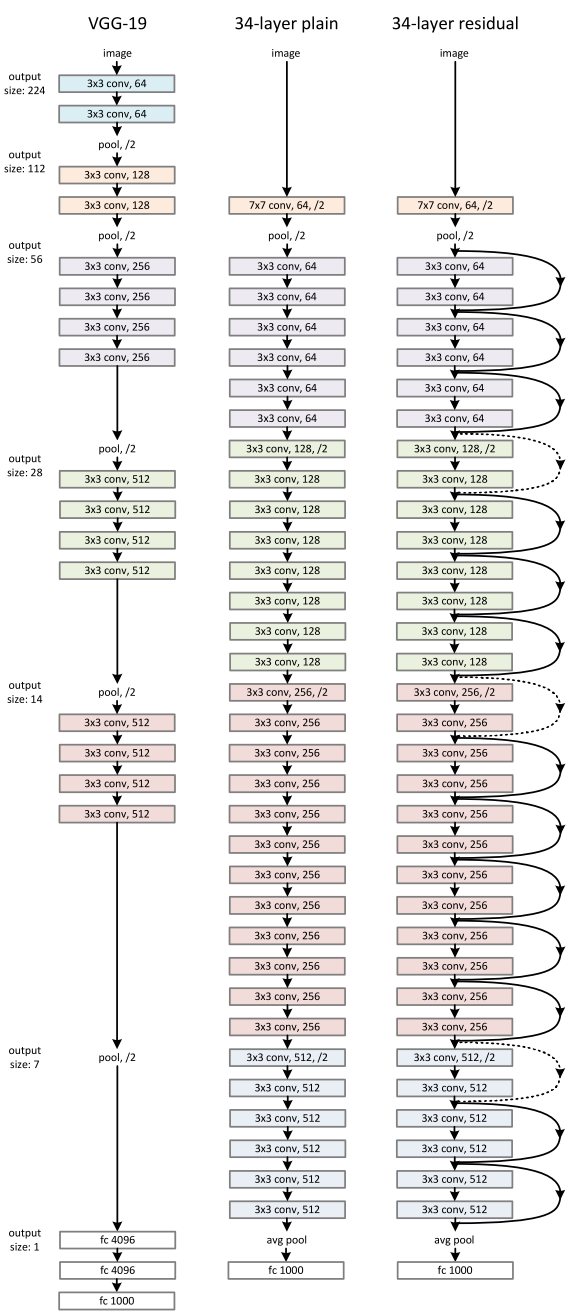
\includegraphics{resnet}
    \caption[]{Comparison of VGG19 architecture and ResNet architecture.}
    \labfig{resnet}
\end{marginfigure}

\section{Generators \& Decoders}
Decoders and generators are meant to generate images or high-dimensional representations from low dimensional input.
For decoders the relation between input and output is often known, upscaling an image in a specific way.
If there are no specific relations between input and output (input is noise), decoders are rather called generators.

Often the architecture for both is inverse to that of classifiers.
The input is first processed by fully connected layers and then rearranged such that it can serve as an input to a convolutional layer.
In contrast to classifier architectures like VGG16, feature decoders upsampling layers.
Upsampling can be achieved through established upscaling methods like nearest neighbor upscaling, bilinear upscaling or bicubic upscaling.
Sometimes transposed convolutions or subpixel upscaling are employed, although they add additional weights to be trained.

Usually, generators mirror the relation of scaling, channel size and number of convolutional blocks of VGG networks but in an inverse direction.

Both decoders and generators are more often used in larger structures like auto-encoders or adversarial networks than as stand-alone networks.

\section{Auto-Encoders}
Auto-encoders combine decoders with encoders.
Encoders are similar to classifiers but instead of returning a class, they return a broader lower resolution representation of its high-resolution input.
This is the inverse to a decoder's job.
Auto-encoders combine an encoder with a decoder such that the low dimensional output of the encoder acts as input to the decoder.
The decoder than tries to reconstruct the original input as good as possible.
For this reason the encoder must compress all the information it gets as an input, such that the decoder can reconstruct the same information from the compressed representation.

The main goal of auto-encoders is to learn such a compressed/more efficient representation that still holds all relevant information.
A very common use-case for auto-encoders are images of faces.
Usually these faces are pre-processed such that they are always aligned similarly in every image.
Then a lower dimensional representation only needs to represent \eg the eye-color since the position of the eyes should be the same in all images.\\
This example also points out another goal of auto-encoders, which is to make the compressed representation interpretable and/or controllable.
This would mean, changing one parameter in the \textbf{feature space} \ie the lower dimensional representation will equate to changing the color of the hair.

The now introduced features space allows for lots of research such as metric learning.

A popular variant of auto-encoders are \textbf{variational auto-encoders (VAE)}.
VAEs add an additional sampling step between the output of the encoder and the decoder.
Thus, the encoder predicts means and standard deviations each dimension in feature space.
These parameters are then used to adjust a multi-dimensional Gaussian distribution from which the inputs of the decoder are sampled.

Such an additional layer of stochasticity is meant to solve a huge short-coming of auto-encoders.
The features space of auto-encoders is often highly specific to the data.
This means that there are many places in feature space which are not explored during training and it is not easy to find the meaningful areas in feature space.
Taking such an undefined feature representation decoder input would result in equally undefined output.
Thus, it is hard to find valid feature representations without using the encoder.

By adding a sampling layer in VAEs, the decoder is suddenly forced to deal with stochastic inputs.
This means that any point in feature space could be an input by pure chance.
Thus, the decoder gets more robust against various feature inputs.
To further reinforce such a behavior, and additional constraint is put on the sampling parameters, that the encoder predicts.
The sampling parameters should be as close to a standard Gaussian ($\mu = 0, \sigma = 1$) as possible.
This is enforced by calculating the Kulback-Leibler Divergence between the encoder output and a standard Gaussian.
\marginnote{The Kulback-Leibler divergence is a measure for two distributions how much they differ.
For two Gaussian distributions, the Kulback-Leibler divergence takes a well-defined form entirely depending on $\mu_1, \sigma_1$ and $\mu_2, \sigma_2$~\cite{KLdiv}.}
The resulting network then allows to generate samples with the decoder and explore the feature space more easily.

\section{Generative Adversarial Networks}
Generative adversarial networks (GAN) were presented by \citeauthor*{GAN} in \citeyear{GAN}~\cite{GAN}.
Nowadays, GANs are widely acclaimed and build the foundations for many approached in computer vision and machine learning.
The researches behind GANs were even lauded with the prestigious Turing Award~\cite{turingaward}.
\marginnote{Other researchers claim to have come up with the idea of GANs earlier, which is kind of a hot topic in the machine learning community.
For safety measures the supposedly previous claim shall be cited as well~\cite{schmidhuber}.}

The basic idea behind GANs is to combine a generator with a discriminator.
The generator's job is to generate data from noise.
Ideally, the generated data should fit the data which is present in a data set.
The discriminator ensures, that this is the case by distinguishing generated samples ('fake') from data set samples ('real').
During training, the generator and the discriminator are in constant competition.
While the discriminator tries to better distinguish fake and real data, tries generator to come up with samples that fool the discriminator.
This can be described by the following equation for a generator $G$, a discriminator $D$, some data $x \in X$, and sampled noise $z \in Z$.
\begin{align}
    \labeq{GAN_G}
    G & = \argmin_G \E_Z[\log D(G(z))] \\
    \labeq{GAN_D}
    D & = \argmin_D \E_X[\log D(x)] + \E_Z[\log( 1 - D(G(z)))]
\end{align}
As this game continues the quality of the generated data becomes better until the generated data becomes indistinguishable from real data.
This way, the generator can for instance create images of faces, which have never been seen before, but look just like any other face.
Such a simple principle can be taken even further, which is the reason why GANs can be found pretty much in any field of computer vision nowadays.

\subsection{Flavors of GANs}
Since GANs have had such an impact, there has naturally been more research to improve GANs in general.

Some approached are able to combine GANs with auto-encoders~\cite{AEGAN} or VAEs~\cite{VAE-GAN} and gain performance improvements from this.
Other approaches add relevant information to the noise input and get the generator to act more like a decoder \cite{cGAN}.
Yet other approaches concentrate on improving the loss function, such that GAN training becomes more stable~\cite{WGAN}.
Again, other approaches improve the quality for high-resolution images by generating samples at different scales~\cite{MSG-GAN} or progressively increasing the image scale~\cite{ProGAN, StyleGAN}

\subsubsection{Relativistic GANs}
One particular approach to improving the loss function finds use in this thesis and thus shall be presented.

Relativistic Standard GAN (RSGAN) and Relativistic average standard GAN (RaSGAN) are two implementations presented by \citeauthor*{RGAN}.
\marginnote{Standard GAN means the GAN as presented in \refeq{GAN_G, GAN_D}.}
They claim that by modifying the loss function the stability of training as well as the quality of generated samples can be improved~\cite{RGAN}.

The main idea behind this approach is, that in a standard GAN approach the discriminator is more focussed on classifying real samples correctly.
If the discriminator is to classify all real samples correctly, then there is no more gradient for real samples as $ \E_X[\log D(x)] \rightarrow 0$.
Then the discriminator mostly learns from generated fake samples and probably over-fit these.\\
A relativistic loss function avoids this by measuring the distance between real predictions and fake predictions with a sigmoid function.
\begin{align}
    \labeq{RSGAN_G}
    G & = \argmin_G - \E_{X, Z}[\log(\sigma(D(G(z)) - D(x))] \\
    \labeq{RSGAN_D}
    D & = \argmin_D - \E_{X, Z}[\log(\sigma(D(x) - D(G(z)))] \\
\end{align}
This more symmetric formulation is meant to push the generator closer to generating samples the follow the data distribution.

RaSGAN advances on the idea of RSGAN by reducing the variability that comes from comparing to single samples $x \in X$ and $G(z), z \in Z$.
Instead, the mean of real samples and generated samples is calculated across the mini-batch and then compared to each sample.
\begin{align}
    \labeq{RAGAN_G}
    G & = \argmin_G - \E_Z[\log(\sigma(D(G(z)) - \E_X[D(x)])] \\
    & - \E_X[\log(1 - \sigma(D(x) - \E_Z[D(G(z))])]\\
    \labeq{RAGAN_D}
    D & = \argmin_D - \E_Z[\log(1 - \sigma(D(G(z)) - \E_X[D(x)])] \\
    & - \E_X[\log(\sigma(D(x) - \E_Z[D(G(z))])]\\
\end{align}
This further improves the quality of generated samples in adversarial training.

